%************************************************
\chapter{A real analysis use case comparison}\label{ch:benan} % $\mathbb{ZNR}$
%************************************************
Having described in detail our innovative approach to event simulation, and having applied it to real datasets, we decided to repeat the preliminary selection of a recent analysis to demonstrate the feasibility of our model in a real-case scenario.

\section{The Higgs decay into two muons}
We generated a FlashSim dataset from the Gen-level information of an existing NanoAOD FullSim dataset, discussed in Section \ref{sec:progen}. We then performed the preliminary selection steps of the analysis presented in \cite{Sirunyan_2021}, specifically that of VBF Channel of H$\rightarrow\mu^+\mu^-$, for the reasons discussed previously.
Our reference was the work of the Pisa CMS group, collected \href{https://github.com/arizzi/PisaHmm}{here}\footnote{https://github.com/arizzi/PisaHmm}. The objective was to verify that the selected objects distributions were on par with those obtained from FullSim.

\subsection{Event selection}

First of all, we define the \emph{selected muons} as the muons with:
\begin{outline}
\1 \texttt{Muon\_pfRelIso04\_all} $<0.25$ (isolated);
\1  \texttt{Muon\_mediumId==True};
\1  \texttt{Muon\_pt} $>20$ GeV (energetic);
\1  \texttt{abs(Muon\_eta)} $<2.4$ (directed forward).
\end{outline}

These are all features we would expect from a pair of muons decaying from a Higgs. An event is also obviously required to have at least two opposite charged muons.

In a similar way, we can identify \emph{selected jets} as those jets with:

\begin{outline}
\1 \texttt{Jet\_pt} $> 50$ GeV or \texttt{Jet\_pt} $> 25$ GeV and \texttt{Jet\_puId} $>0$ (energetic, non PileUp jets);
\1  \texttt{Jet\_jetId} $>0$;
\1  \texttt{abs(Jet\_eta)} $<4.7$ (forward);
\1 \texttt{Jet\_MuonDr} $>0.4$ (spatially separated from the muons).
\end{outline}

A VBF candidate event is required to have at least two jets respecting the previous properties, one with $p_T>35$ Gev, the other with $p_T>25$ Gev, $m_{jj}>400$ Gev and $\Delta\eta<2.4$. Selected events are further grouped into two independent categories. Events in which the two muons form an invariant mass between 115 and
135 GeV belong to the signal region (VBF-SR), which is enriched in signal-like events. Events with 110 < $m_{\mu\mu}$ < 115 GeV or 135 < $m_{\mu\mu}$ < 150 GeV belong to the mass sideband region (VBF-SB), which in the full analysis has been used as a control region to estimate the backgroung.

For each selected event we define the new, derived quantities. Some crucial ones are:

\begin{outline}
\1 An \emph{Higgs} object given by the sum of the two four-vectors of the selected muons;
\1 Observables sensitive to $p_T$ and angular correlations between muons and jets: The $p_T$\emph{-balance ratio}, defined as:
\[R(p_T) = \frac{p_T^{jj}+p_T^{\mu\mu}}{p_T(j_1) + p_T(j_2) + p_T(\mu\mu)}\]

and the \emph{Zeppenfeld variable} $z^*$, defined from the \emph{rapidity y} as:

\[z^* = \frac{y_{\mu\mu} - (y_{j_1} + y_{j_2})/2}{\abs{y_{j_1} + y_{j_2}}}\]

\1  The azimuthal angle ($\phi_{CS}$) and the cosine of the polar angle ($\cos\theta_{CS}$) computed in the dimuon \emph{Collins–Soper} rest frame \cite{PhysRevD.16.2219}.
\end{outline}

\subsection{A DNN for event classification}
The authors of \cite{Sirunyan_2021} used a deep neural network (DNN) multivariate discriminant, trained to distinguish the expected signal from background events using kinematic input variables that characterize the signal and the main background processes in the VBF-SR. The signal is then extracted from a \emph{binned maximum-likelihood fit} to the inverse hyperbolic tangent of the output of the DNN discriminator simultaneously in the VBF-SR and the VBF-SB regions. 

We recovered the \emph{exact same network} as the one used in the final publication, with the final weights and parameters resulting from the trainings already performed by the authors of the original paper on the FullSim dataset. We tested the network on our FlashSim data to compare the ouput with the one on the FullSim datasets used in the analysis and taken as Gen-level truth for generating our samples.

The network takes as input 25 variables. The first 23 are listed below:

\begin{outline}
\1 Six variables associated with production and decay of the dimuon pair: its mass $m_{\mu\mu}$, the absolute and relative mass resolutions $\Delta m_{\mu\mu}$, $\Delta m_{\mu\mu}/m_{\mu\mu}$, its momentum $p_T^{\mu\mu}$ and its logarithm, the pseudorapidity $\eta_{\mu\mu}$;

\1 The azimuthal angle ($\phi_{CS}$) and the cosine of the polar angle ($\cos\theta_{CS}$), the $p_T$\emph{-balance ratio} $R(p_T)$ and the logarithm of the \emph{Zeppenfeld variable} $z^*$;

\1 The vector components of the leading jets, $p_T(j_1)$, $\eta(j_1)$, $\phi(j_1)$, $p_T(j_2)$, $\eta(j_2)$, $\phi(j_2)$, and their QGL scores, $QGL(j_1)$, $QGL(J_2)$, since jets in signal events are expected to originate from quarks, whereas in the DY process they can also be initiated by gluons;

\1 Key variables referring to the dijet system: its mass $m_{jj}$ and $\log(m_{jj})$, the pseudorapidity distance between the two jets $\Delta \eta_{jj}$;

\1  The minimum distance in pseudorapidity of the Higgs candidate with the two leading jets $\min(\eta(\mu\mu, j_1),\eta(\mu\mu, j_2))$

\1 The data taking year (set to 2018 for both FullSim and FlashSim samples);
\end{outline}

Additionally, the VBF signal events are expected to have suppressed hadronic activity in the rapidity gap between the two leading jets. This feature is exploited by considering \emph{soft jets} in the event that are defined by clustering, via the \emph{anti-}$k_T$ jet-clustering algorithm with a distance parameter of 0.4, charged particles from the primary interaction vertex excluding the two identified muons and those associated with the two VBF jets. The soft jets are required to have $p_T>5$ GeV. The number of soft jets in an event, $N^{\text{soft}}_5$, as well as the scalar sum of their transverse momenta, $H^{\text{soft}}_{(2)T}$, are used as additional input variables. 
Because soft activity depends upon the presence of additional charged particles, which we have not been simulated in the present FlashSim work, we resorted to fixing the values of these two variables to $N^{\text{soft}}_5=0$ and $H^{\text{soft}}_{(2)T}=1.0$ GeV. As we are interested in performing a comparison of the DNN output for FullSim and FlashSim, using fixed values in the evaluations of both does not impair the results.

\section{FullSim vs FlashSim}

We observe good results on distributions directly related to the simulated targets of FlashSim, even on samples such as EWK which were not seen byt the NF networks during training. Figure \ref{fig:selmuonpt} shows the $p_T$ for muons, which present negligible deviation when compared to the FullSim sample. The bottom panel shows the ratio between the FlashSim and the FullSim sample, were the chosen convention here and in the following has been to always divide by the FullSim.

\begin{figure}
    \centering
    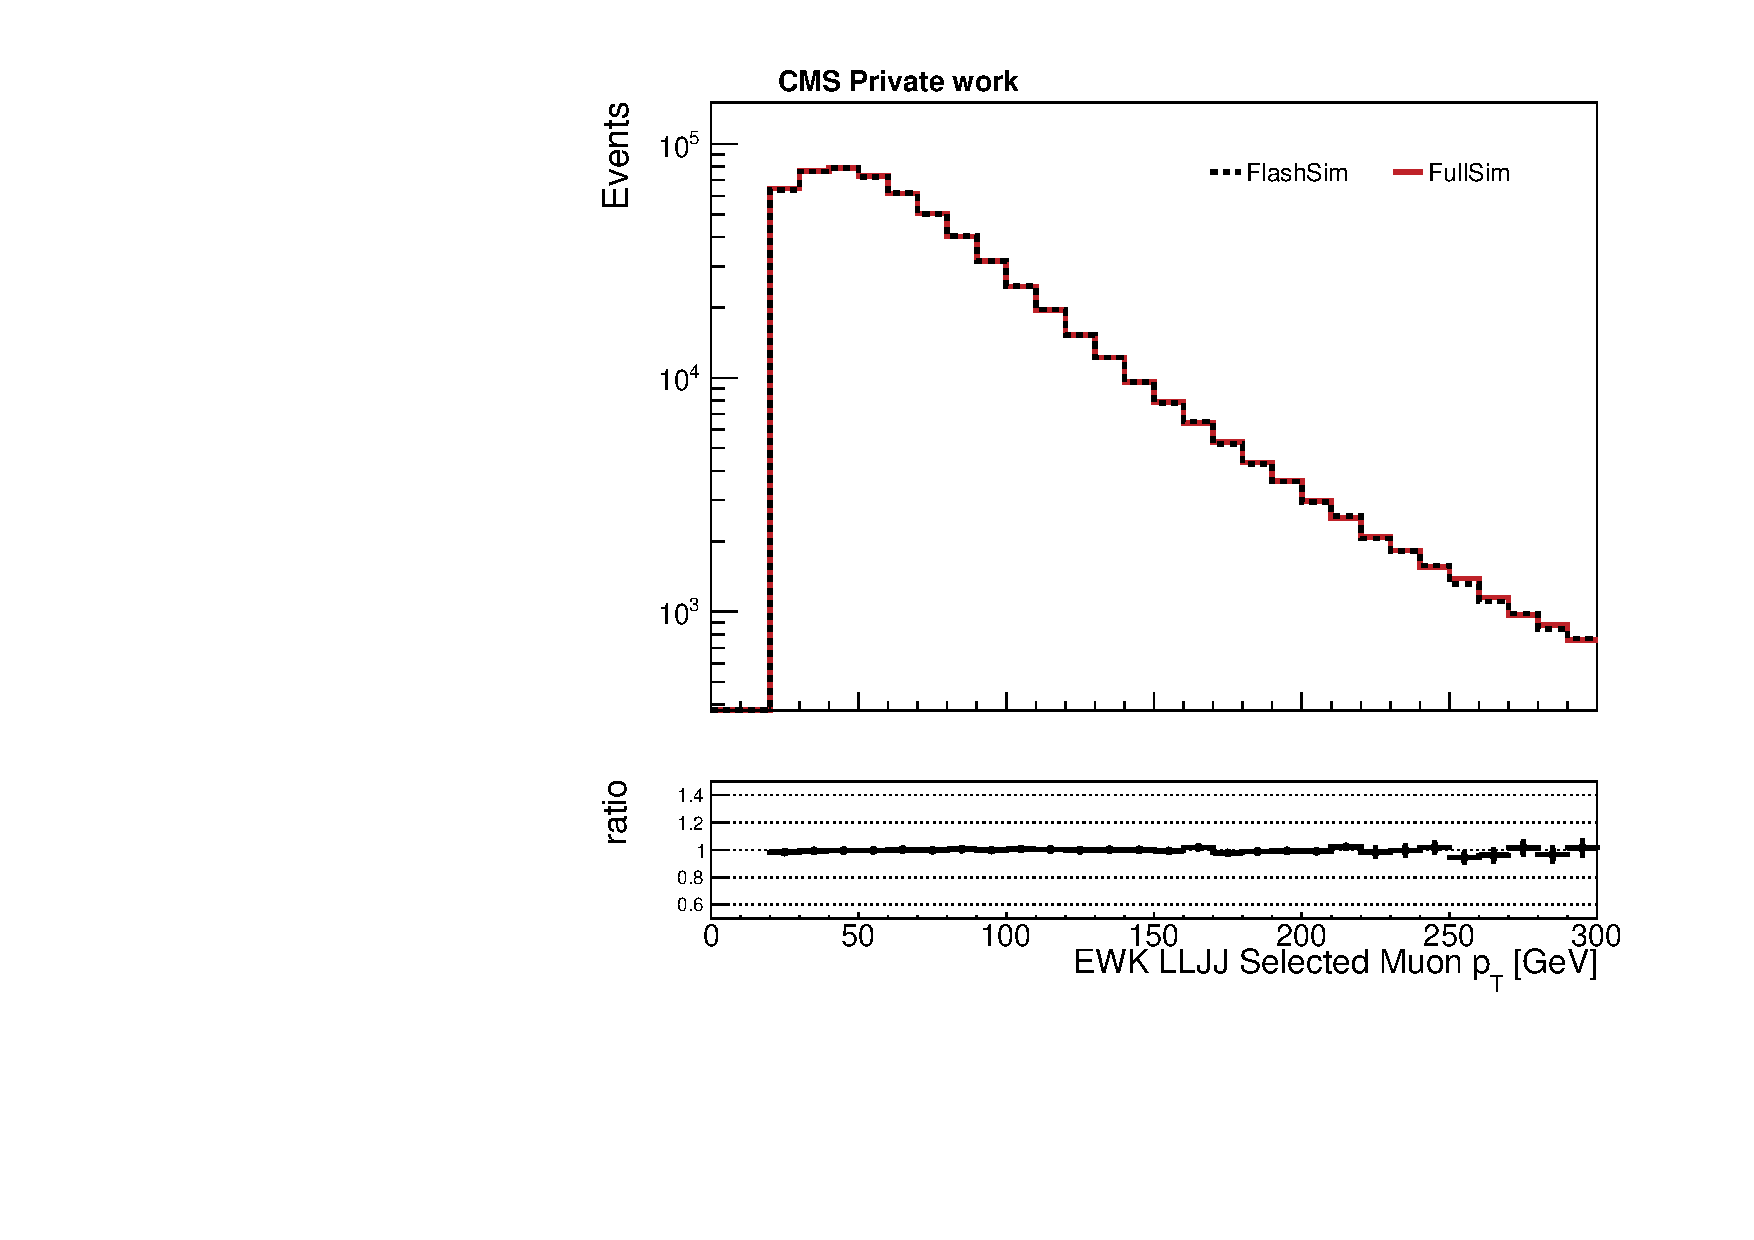
\includegraphics[width=\linewidth]{gfx/ch6/EWK_LLJJ_SelectedMuon_pt____log.pdf}
    \caption[Selected muon $p_T$]{There is close agreement for the selected muons between FullSim and FlashSim}
    \label{fig:selmuonpt}
\end{figure}

However, for jets, the agreement is not as good as for muons. Figure \ref{fig:j1pt} shows that the $p_T$ for the second selected jet is not as high for FlashSim jets as it is for FullSim ones. We tried to explain this result by remembering that our FullSim is missing \emph{fakes} jets due to noise and PileUp, present in the other sample. In principle, higher-$p_T$ fake jets may be selected in place of the second event jet for some of the FullSim samples, explaining the deviation observed. 

\begin{figure}
    \centering
    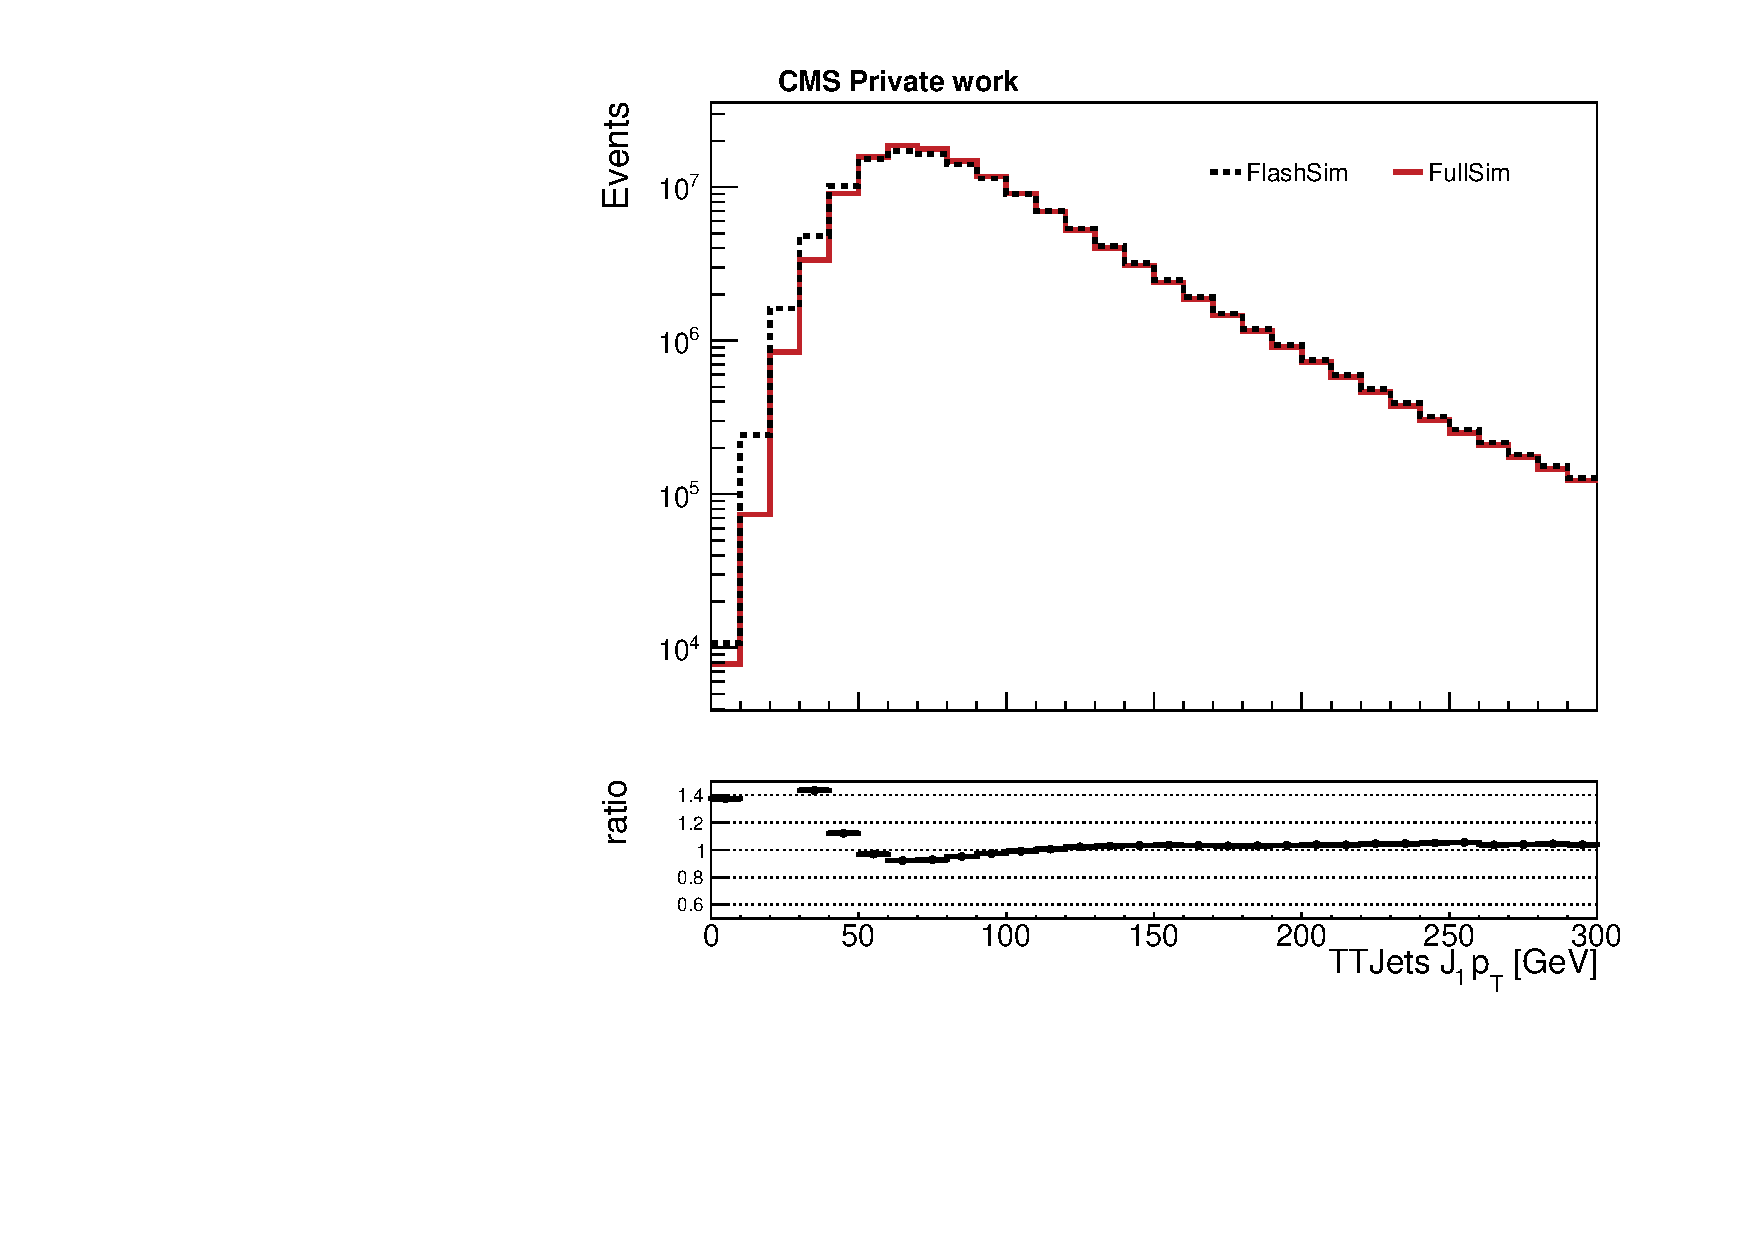
\includegraphics[width=\linewidth]{gfx/ch6/TTJets_J1_pt____log.pdf}
    \caption[J$_1$ $p_T$]{Perhaps because of the absence of \emph{fakes}, we see some disagreement between the two samples, as the FlashSim jets are softer and less energetic than FullSim ones.}
    \label{fig:j1pt}
\end{figure}

The distributions related to angular distributions also show a good performance. We plot in Figure \ref{fig:angulardist} the histograms for the Signal vs DY processes, to show how these variables can be \emph{discriminant} in distinguishing between signal and background.

\begin{figure}
    \myfloatalign
    \subfloat[]
    {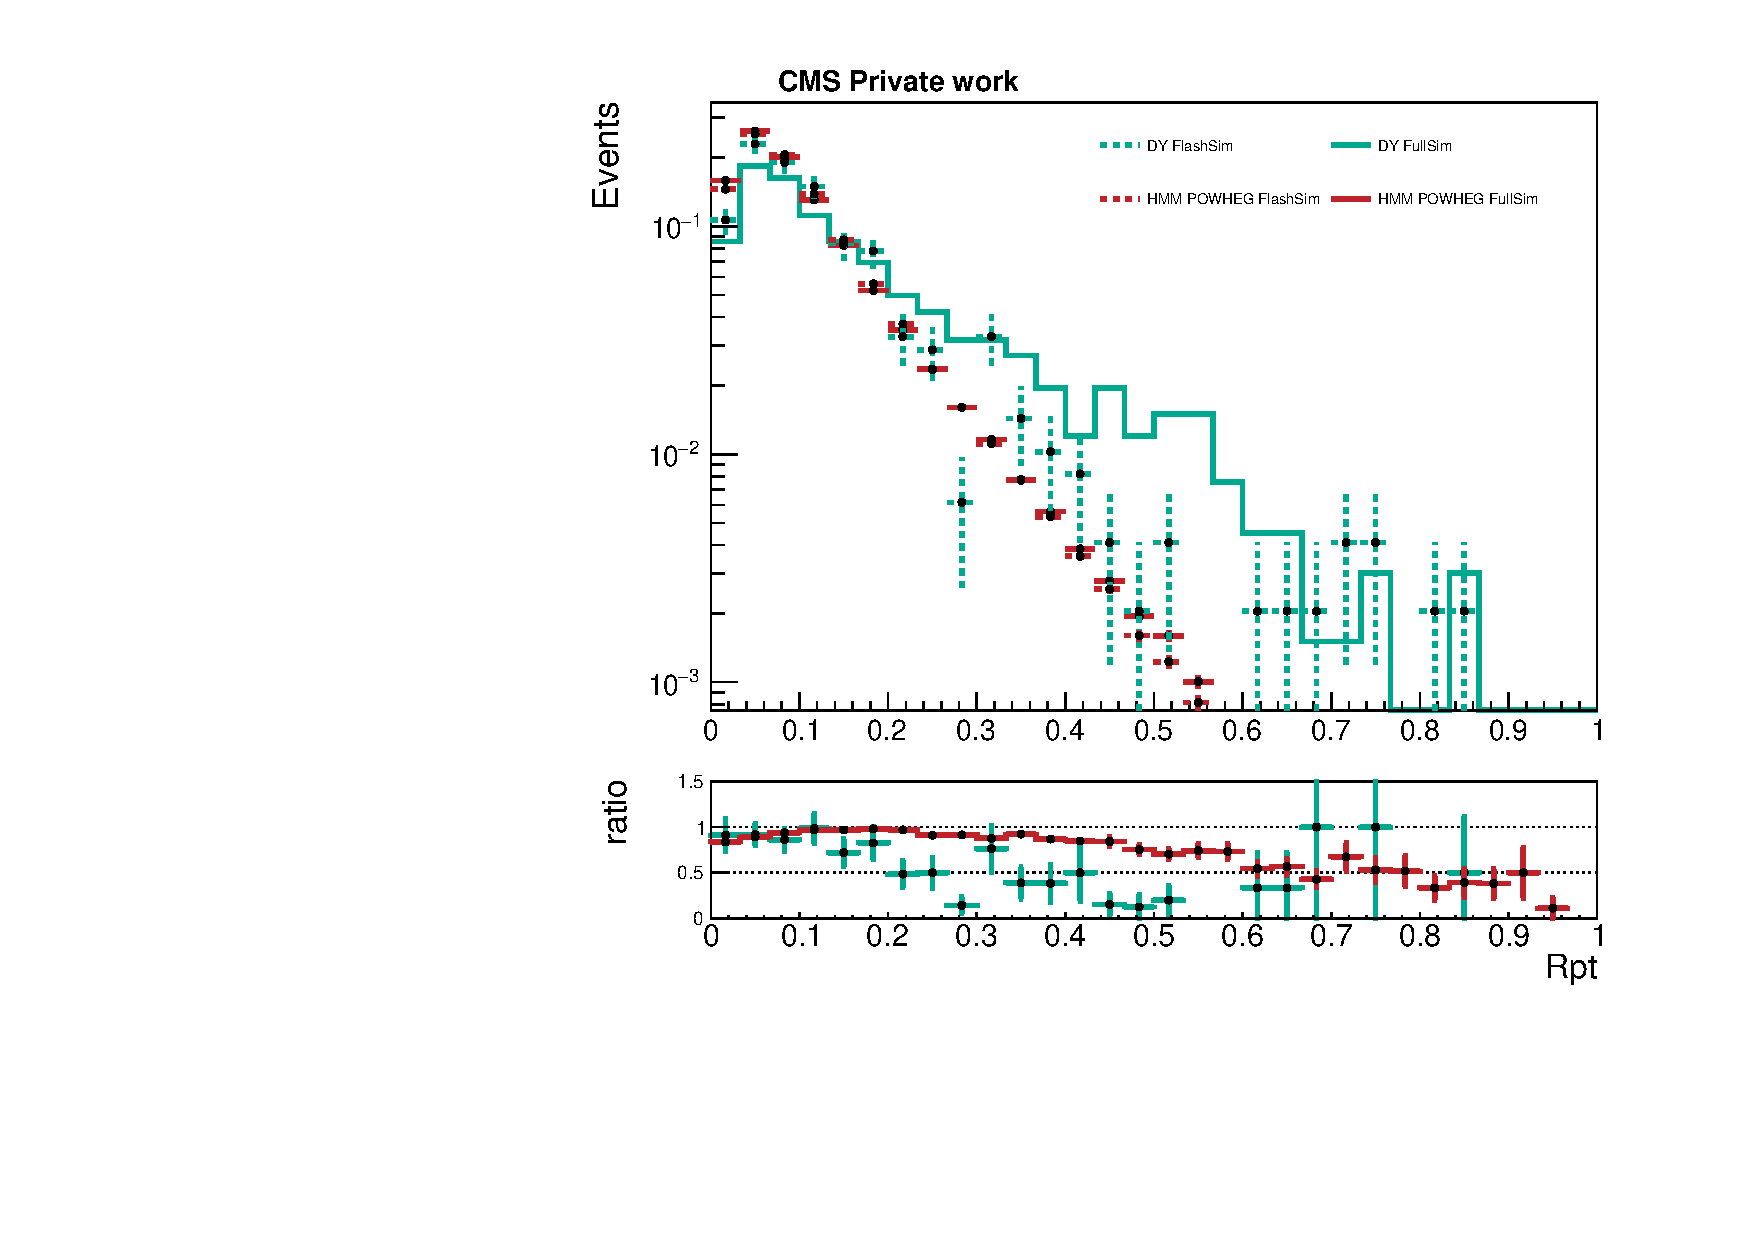
\includegraphics[width=\linewidth]{gfx/ch6/DY2Jets_vs_HMM_powheg_Rpt___SignalRegion_log_normalizedc2.pdf}}\\
    \subfloat[]
    { 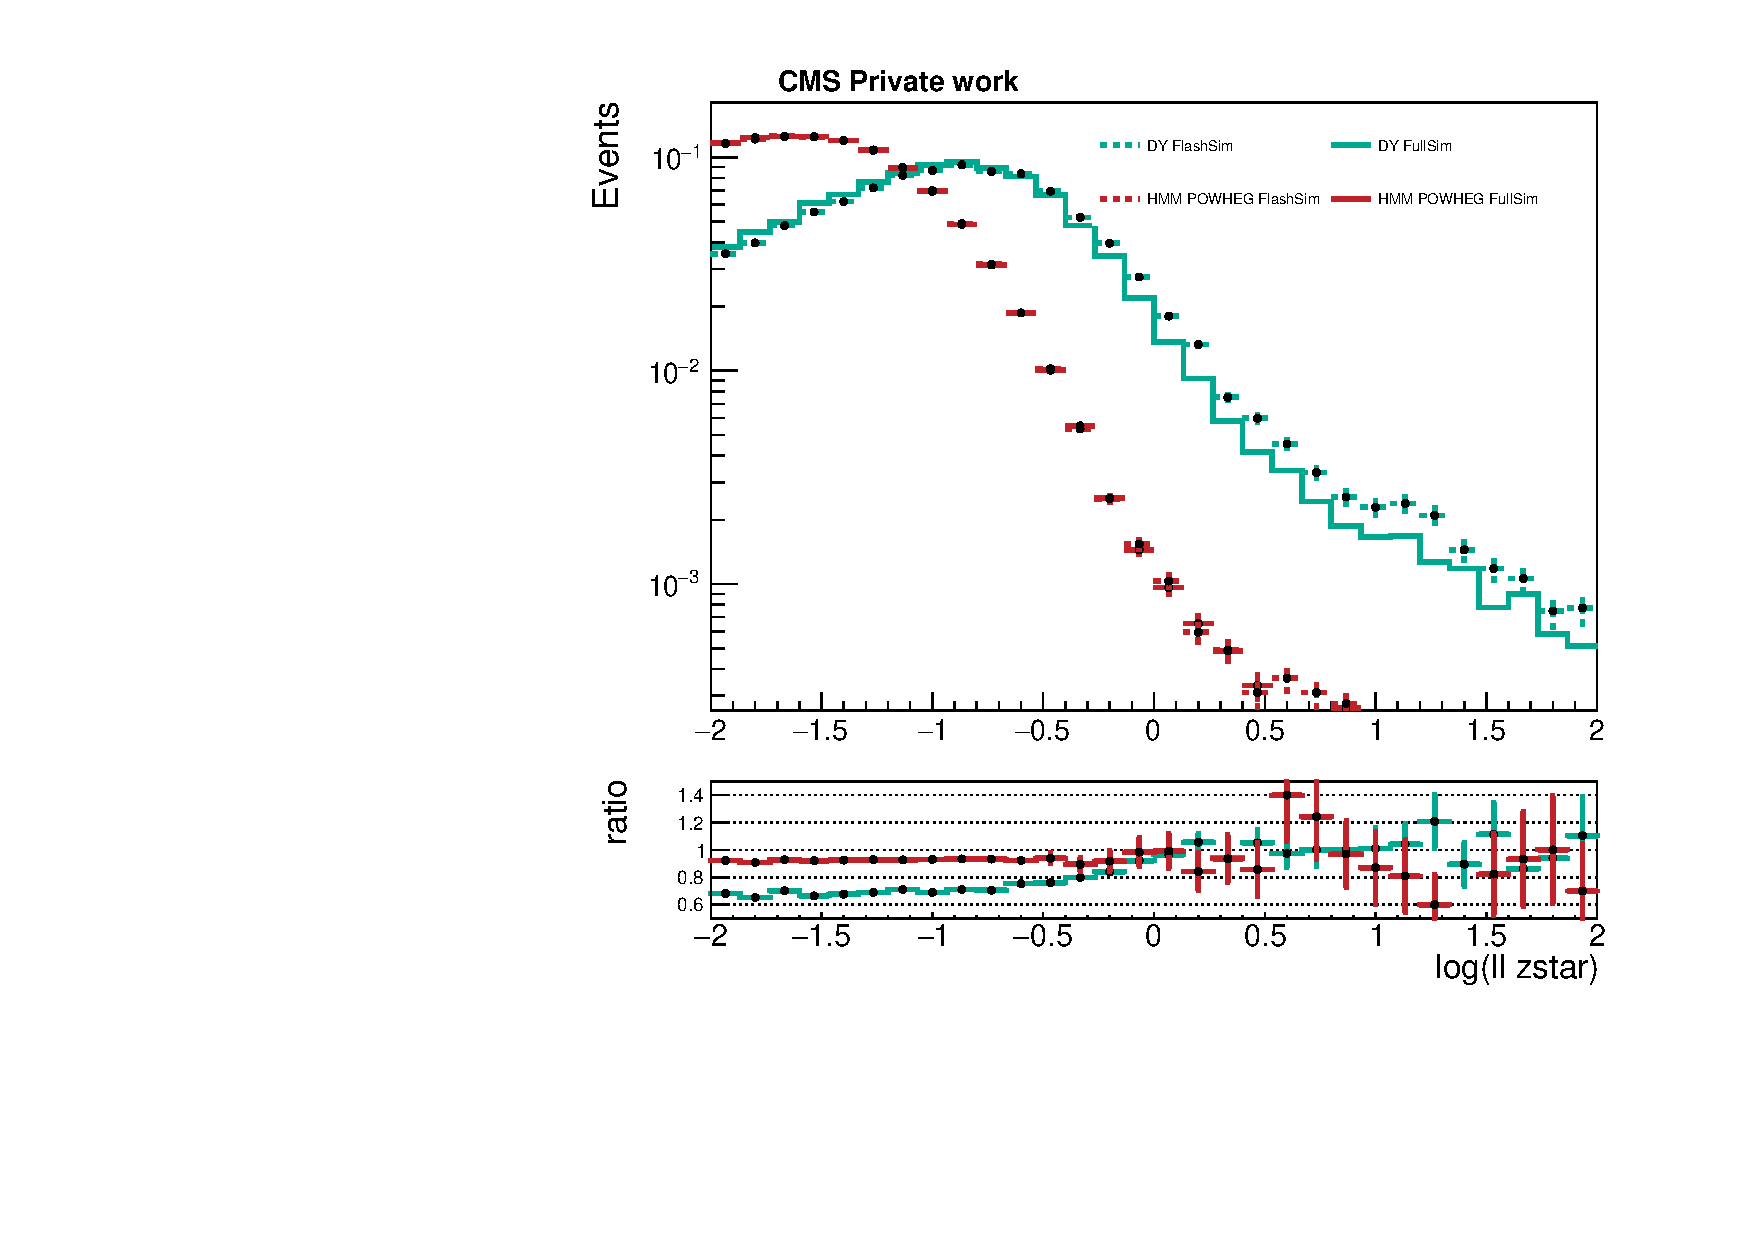
\includegraphics[width=\linewidth]{gfx/ch6/DY2Jets_vs_HMM_powheg_ll_zstar_log___PreSel_log_normalized.pdf}} 
    \caption[Angular distributions]{ (a) The R($p_T$) distribution in the Signal region also shows that FlashSim is struggling with the tails of the DY process, previously unseen during training. (b) The log($z^*$) (for the pre-selected objects in both regions) is clearly distributed differently for the two processes.}\label{fig:angulardist}
    
\end{figure}

We show in Figure \ref{fig:DNNout} the outputs of the VBF DNN discriminator network for each single process, which was used as the fit function for the real analysis.

\begin{figure}
    \myfloatalign
    \subfloat[]
    {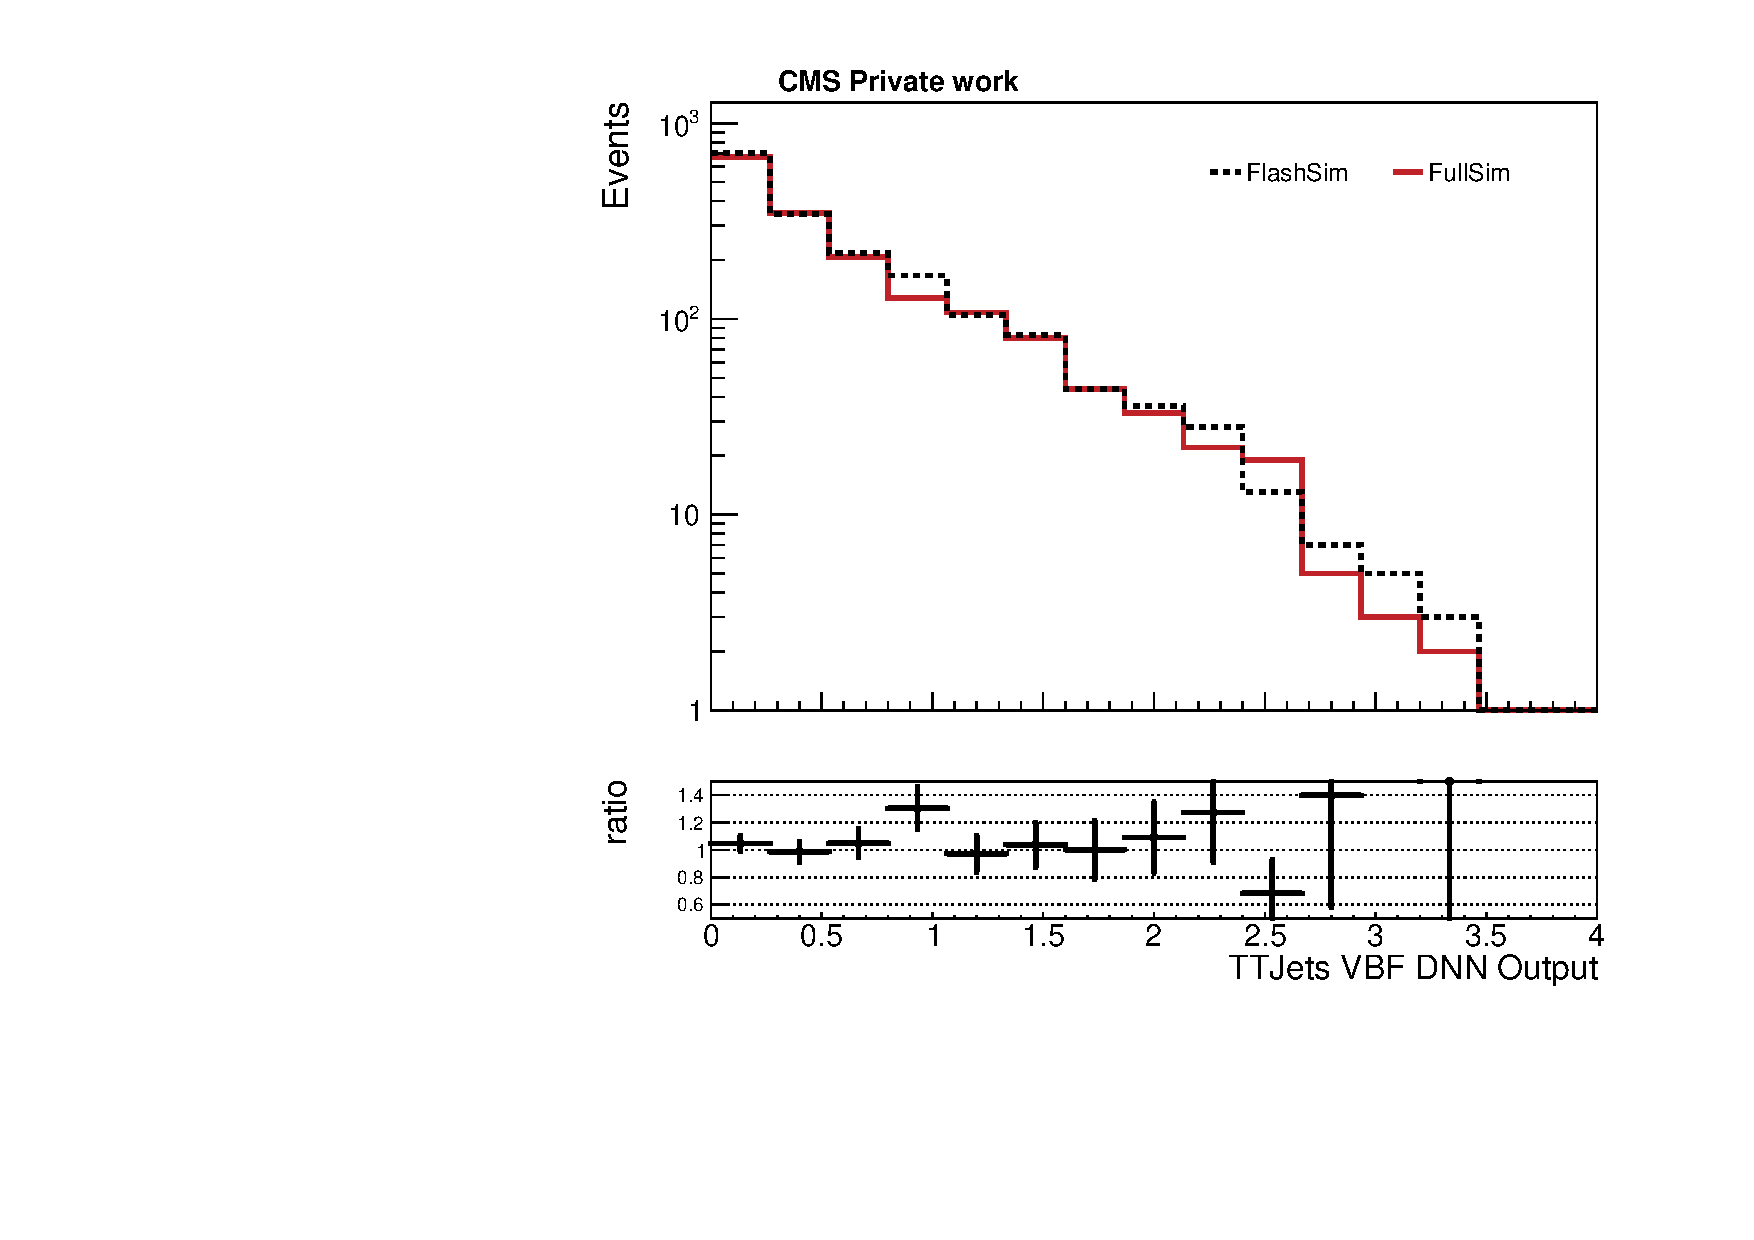
\includegraphics[width=0.45\linewidth]{gfx/ch6/TTJets_DNN18Atan___SignalRegion_log.pdf}}
    \subfloat[]
    { 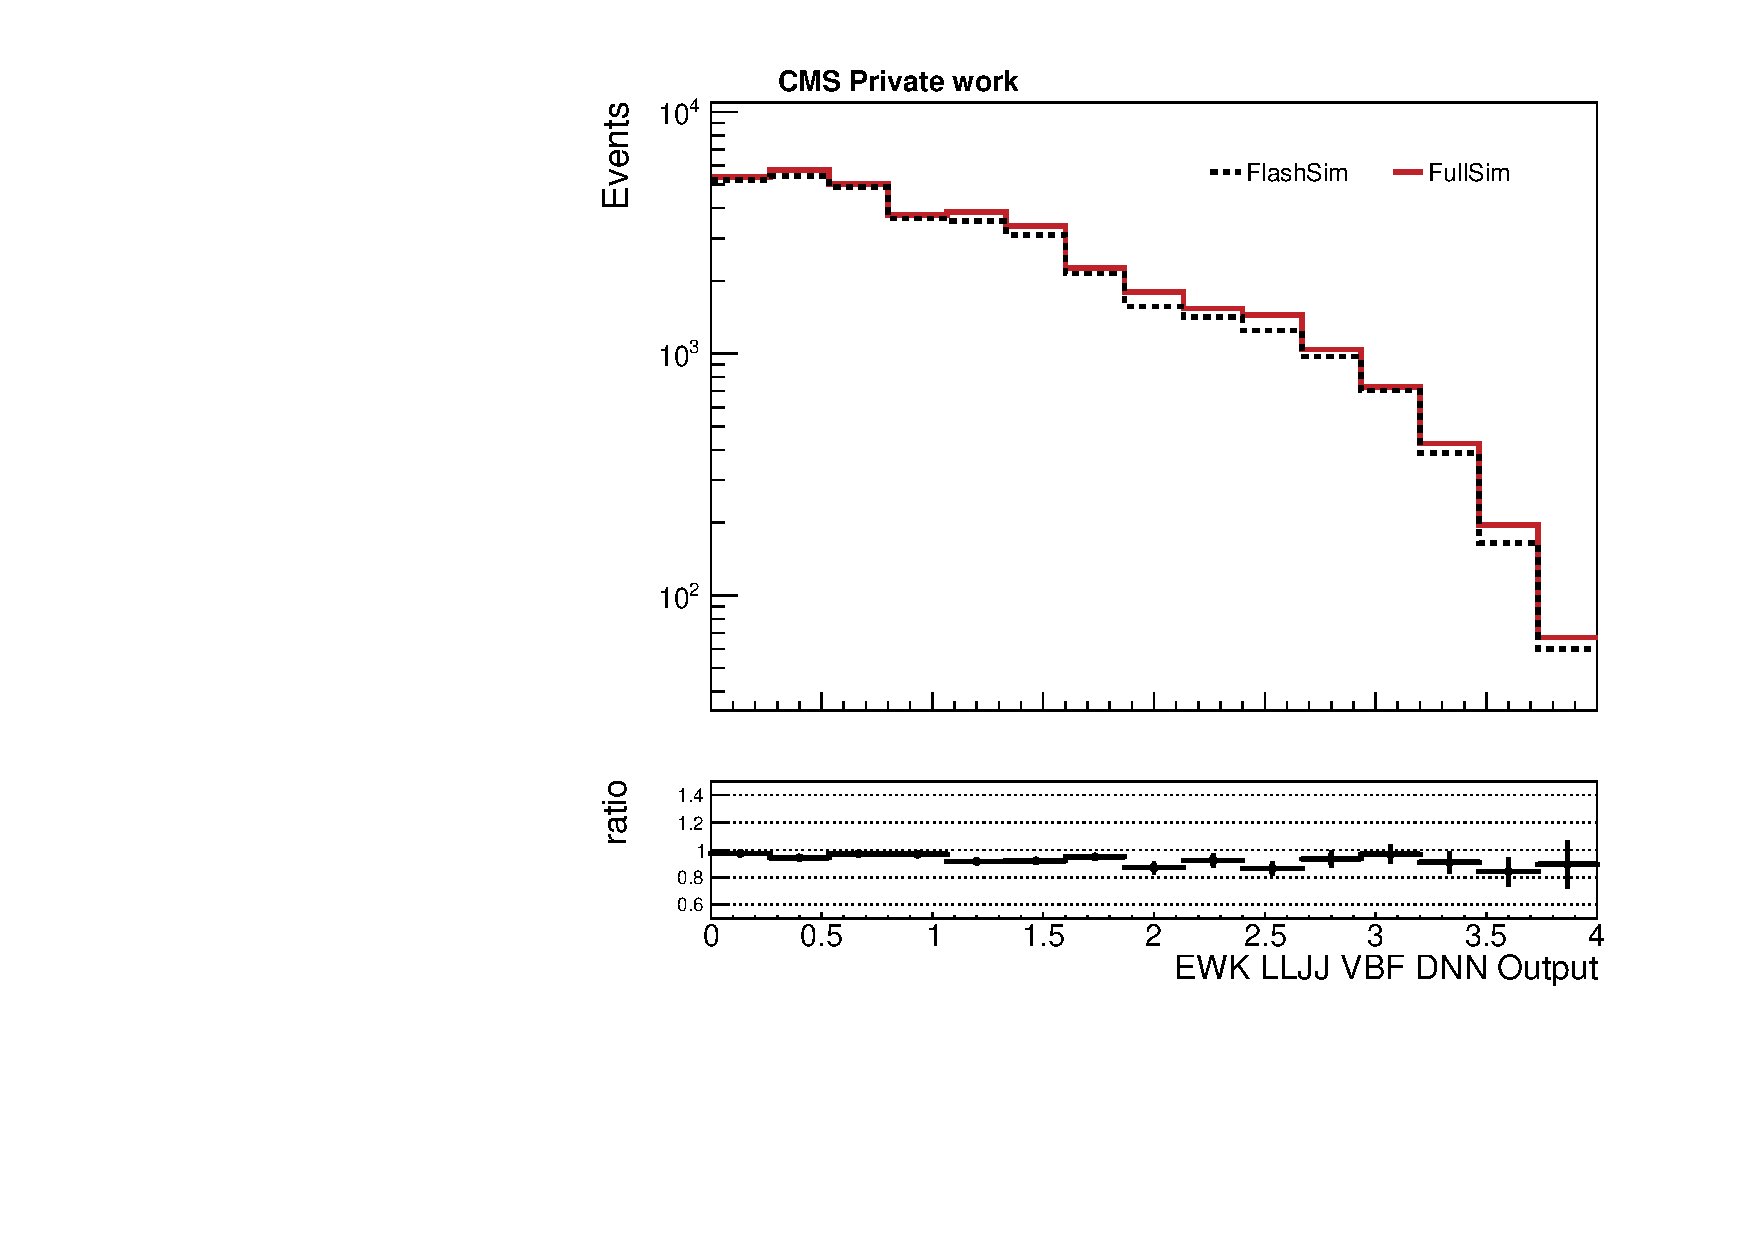
\includegraphics[width=0.45\linewidth]{gfx/ch6/EWK_LLJJ_DNN18Atan___SignalRegion_log.pdf}}\\
    \subfloat[]
    {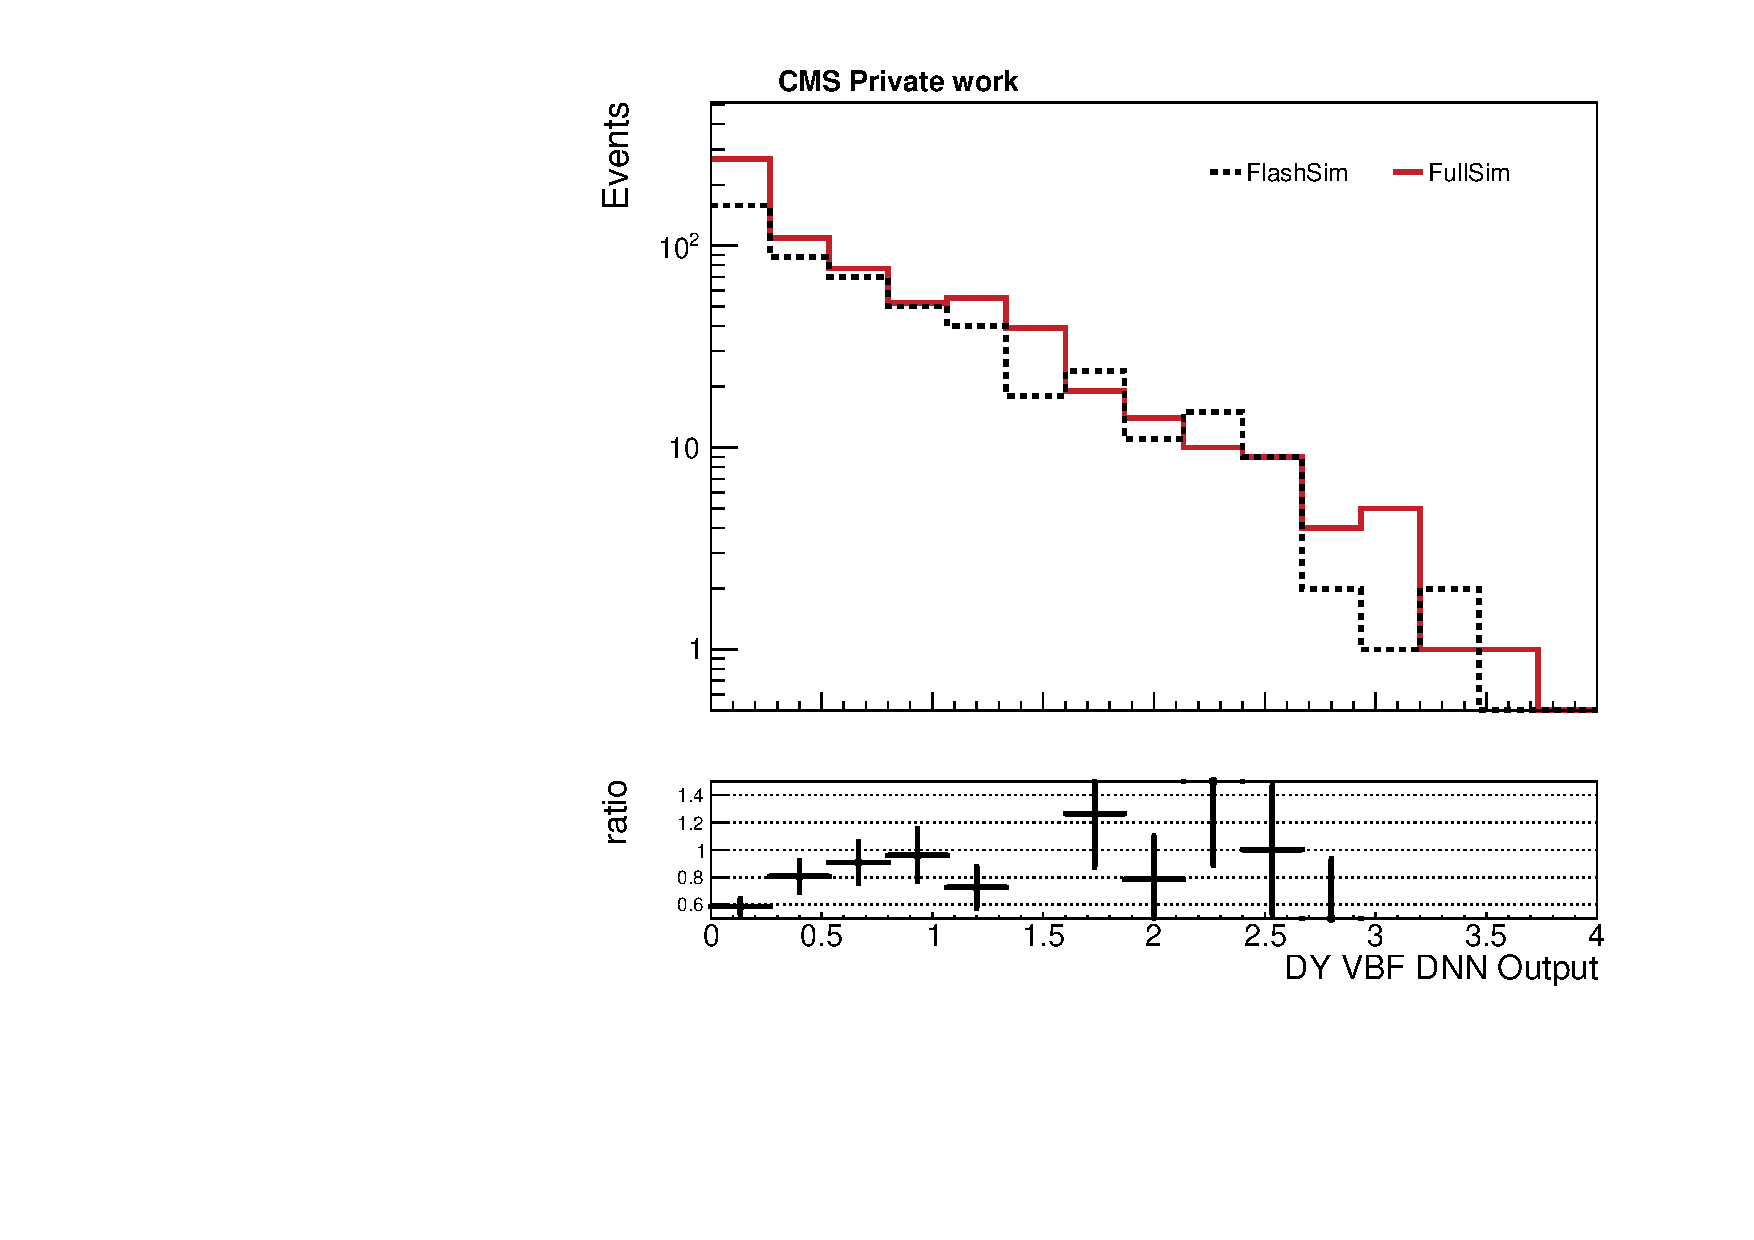
\includegraphics[width=0.45\linewidth]{gfx/ch6/DY2Jets_DNN18Atan___SignalRegion_log.pdf}}
    \subfloat[]
    { 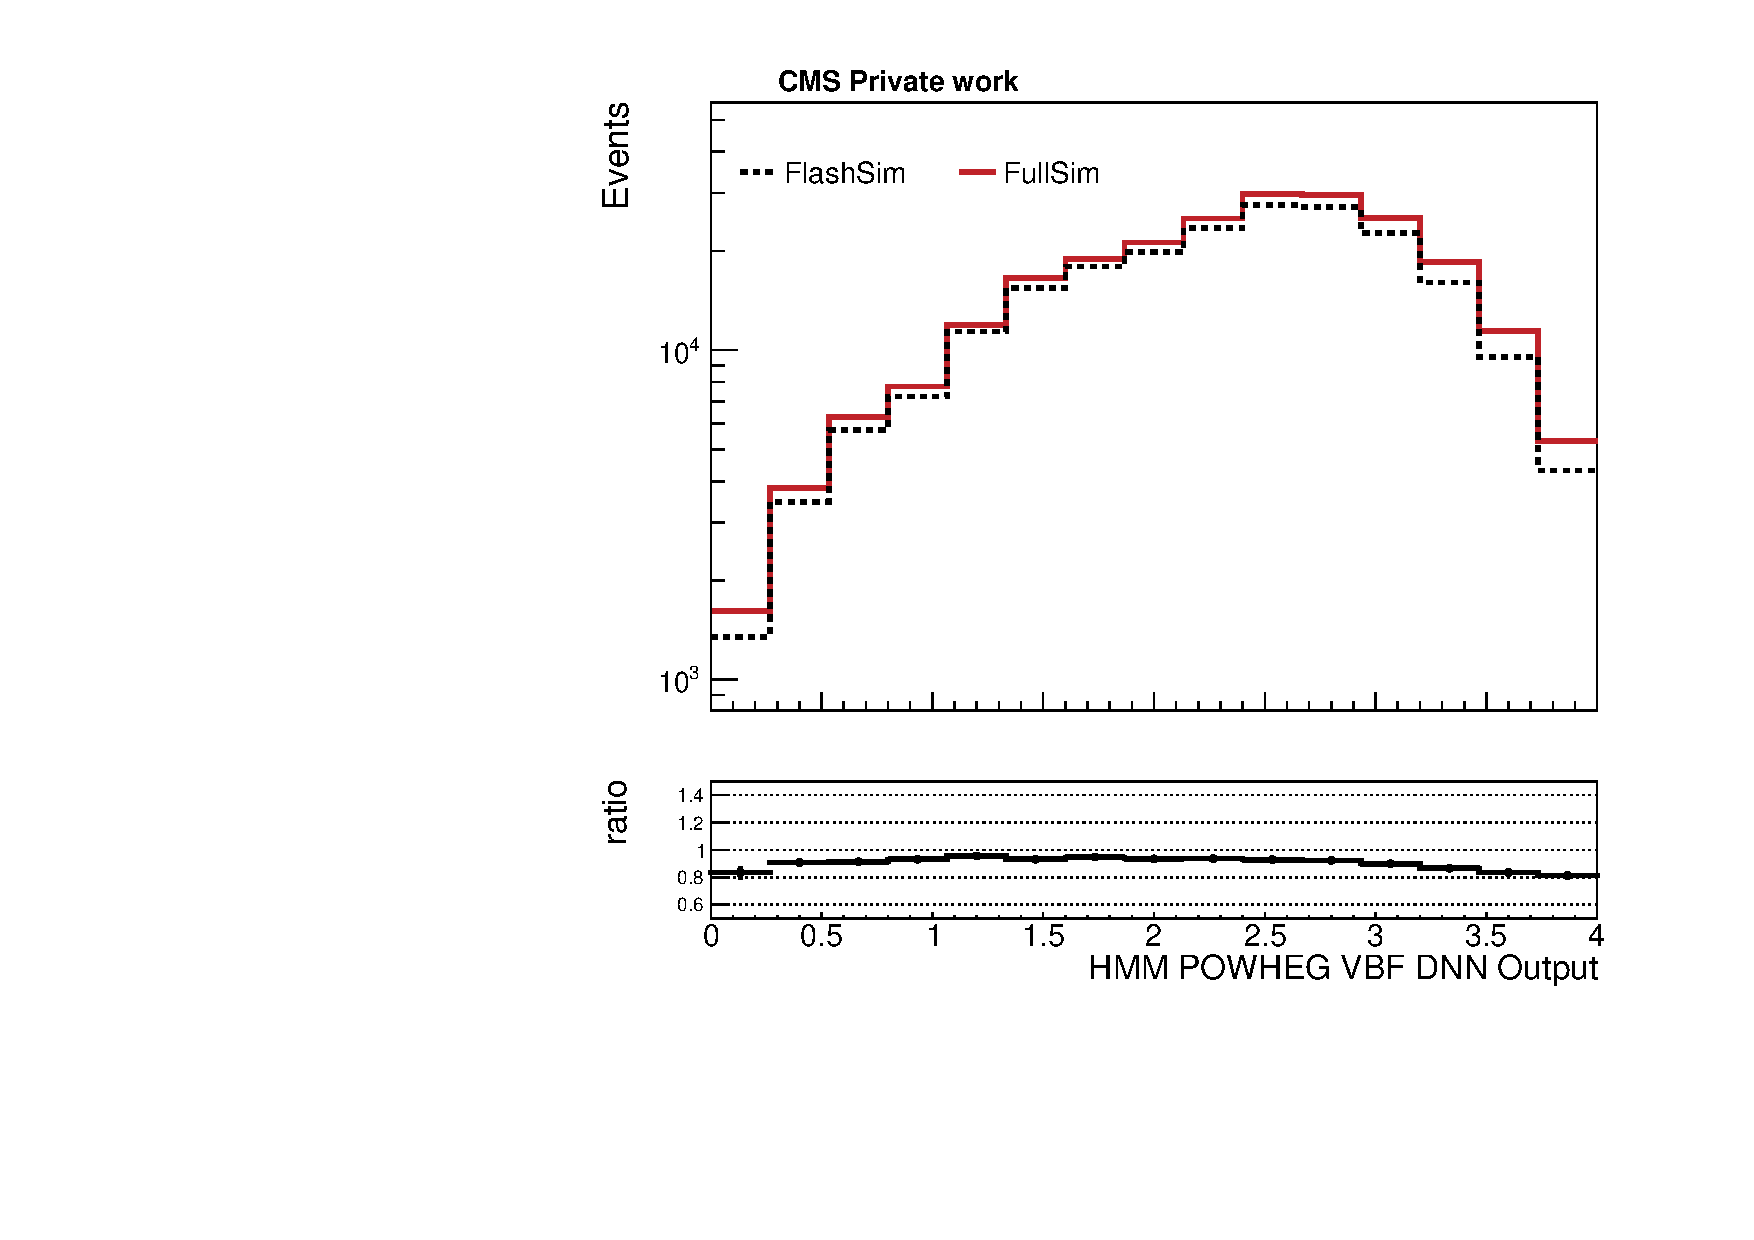
\includegraphics[width=0.45\linewidth]{gfx/ch6/HMM_powheg_DNN18Atan___SignalRegion_log.pdf}} \\
    \subfloat[]
    { 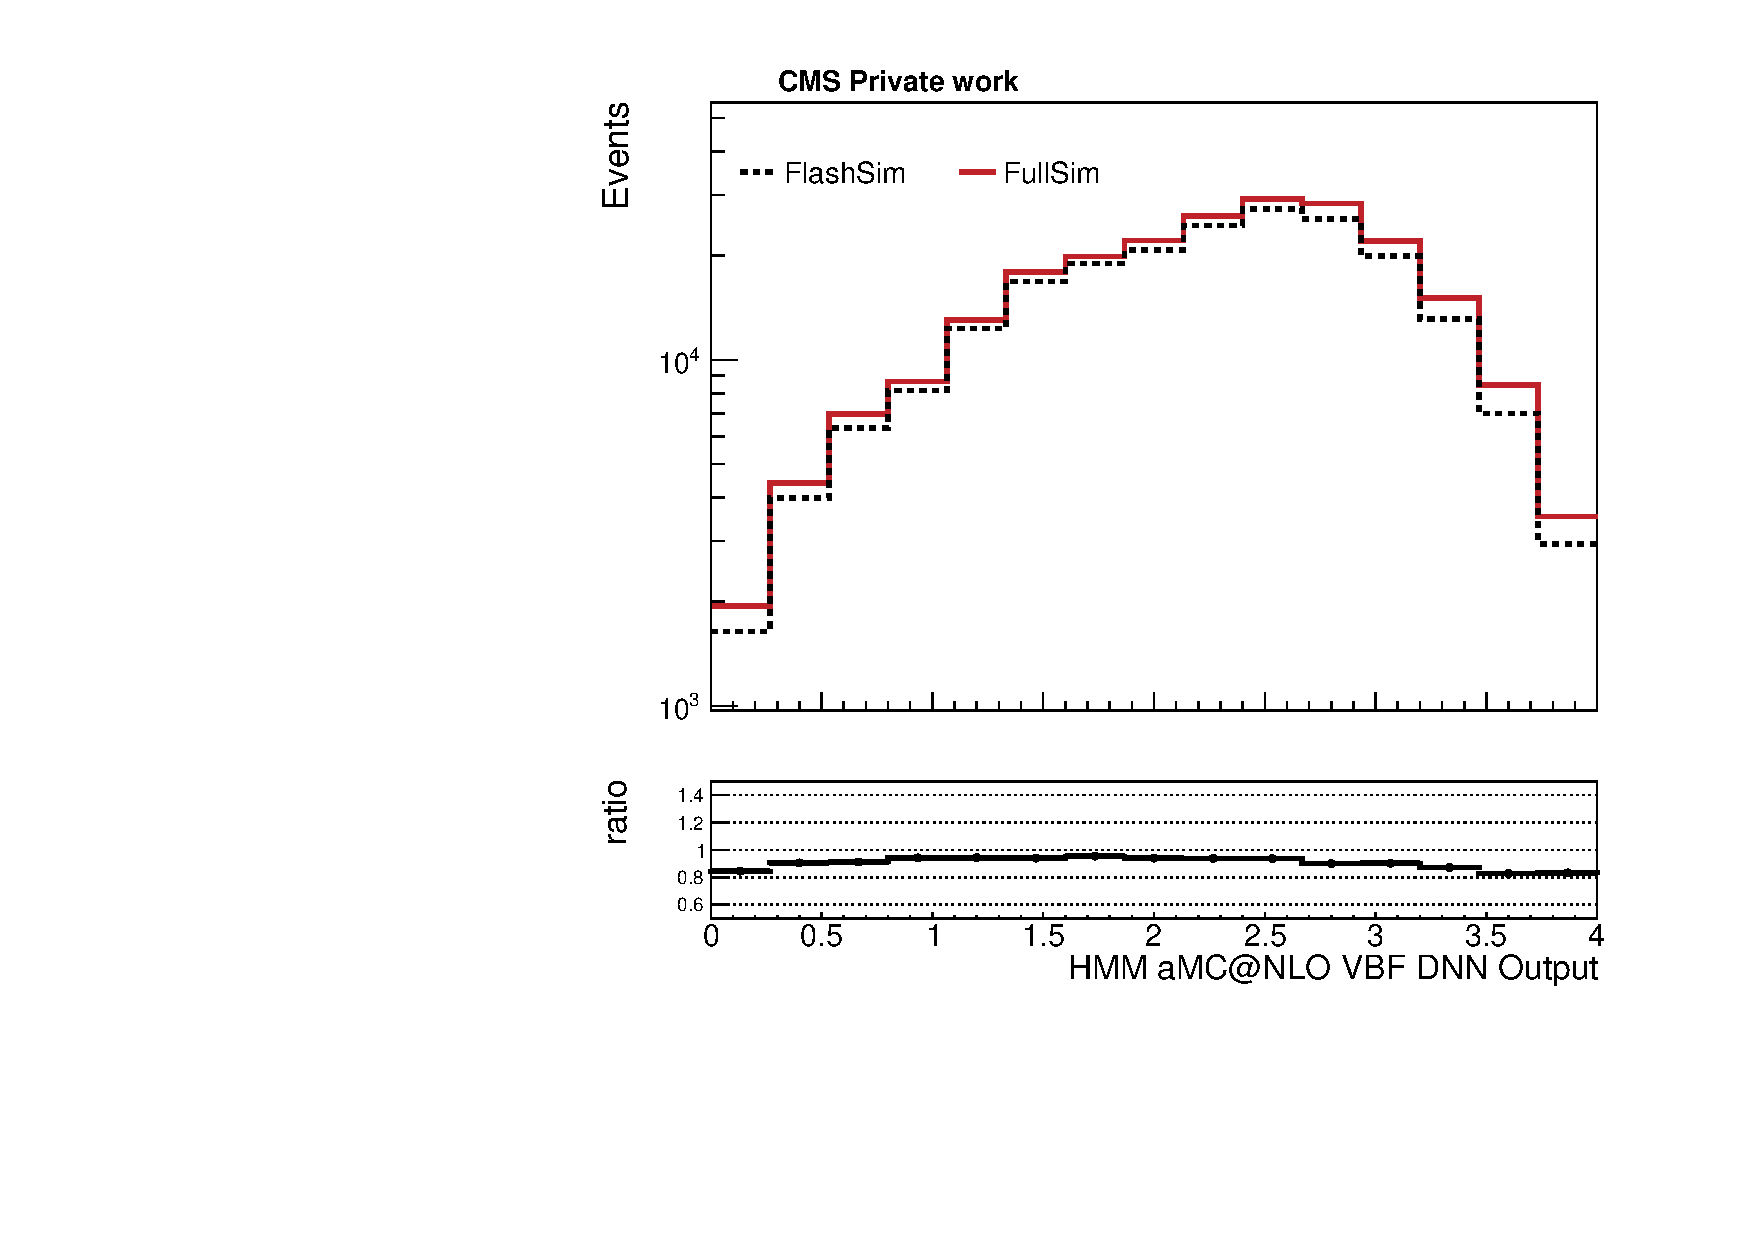
\includegraphics[width=0.45\linewidth]{gfx/ch6/HMM_amcatnlo_DNN18Atan___SignalRegion_log.pdf}}
    \caption[Angular distributions]{Background processes, such as (a), (b), and (c) are always decreasing, while signal processes ((d) and (e)) are increasing in the 0,3 range. All outputs are from data passing the pre-selection and being in the Signal region. }\label{fig:DNNout}
\end{figure}

Finally, a very interesting property of our approach that we wish to verify is the ability of handling the calculation of \emph{theoretical variations} between two samples of the same process. This is the case, for example for the two samples of the signal datasets, which differ in the theoretical technique employed for \emph{systematic inclusion of higher order QCD effects}: one employed the \texttt{POWHEG} method \cite{Nason_2004}, the other the \texttt{MadGraph5\_aMC@NLO} \cite{powpow} one. Suppose we had a FullSim variation $V^1_{Full}$, we computed its FlashSim $V^1_{Flash}$ sample as well as that of another possible variation $V^2_{Flash}$. We would expect that the actual $V^2_{Full}$ may be reobtained faster by the factorization:

\[V^2_{Full} = V^1_{Full} \frac{V^2_{Flash}}{V^1_{Flash}}
\]

as the ratio factors out the FlashSim differences and leaves out only the 2/1 sample differences which are then multiplied by the $V^1_{Full}$ sample. Figure \ref{fig:sysvar} shows that our expectations are met by the FlashSim approach, as the aMC@NLO FullSim variation sample agrees with the ratio calculated from the POWHEG variation sample and the aMC@NLO FlashSim sample. This opens up the way to fast calculations of theoretical variations starting only from a single, pre-existing FullSim sample, implying a considerable speed-up when compared to re-starting always from Gen-level, as it is currently the case.

\begin{figure}
    \centering
    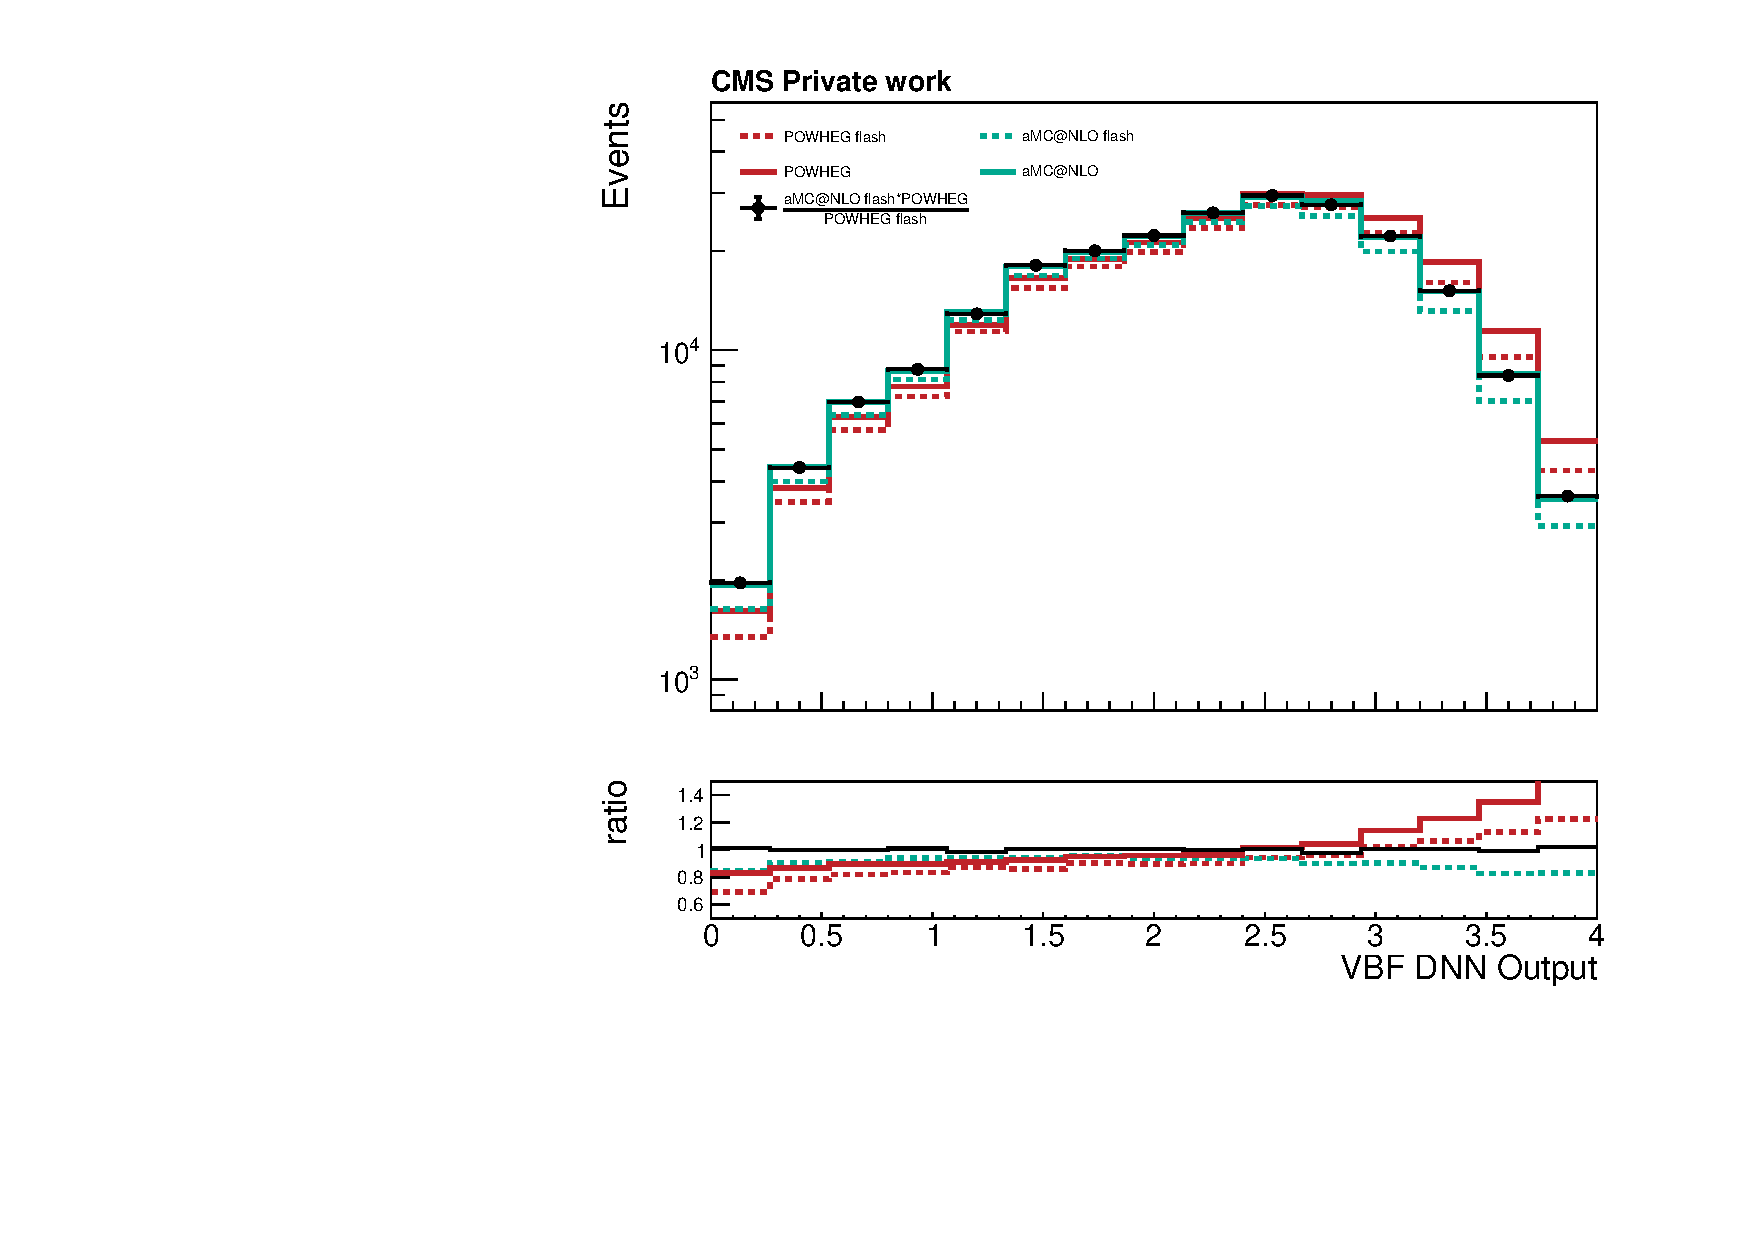
\includegraphics[width=\linewidth]{gfx/ch6/systematic_production.pdf}
    \caption[Systematic production]{The aMC@NLO FullSim systematic variations can be reobtained from the FlashSim simulation and a POWHEG sample--the solid green line and the black dots coincide.}
    \label{fig:sysvar}
\end{figure}

\section{FlashSim vs Gen}

A final test for the goodness of the proposed simulation approach is the comparison with the Gen-level information. Part of the chosen selection analysis objects may in fact be computed starting from Gen-level information alone, and thus we can ask ourselves if the FlashSim results are significantly different from those obtained with its inputs, the Gen values. In the following, we compare results for the Signal sample considering the three samples of FullSim, FlashSim and Gen.

For the $\log(z^*)$ angular distribution, already very precise at Gen level, Figure \ref{fig:zstargen} shows no significan deviations between the three samples.

\begin{figure}
    \centering
    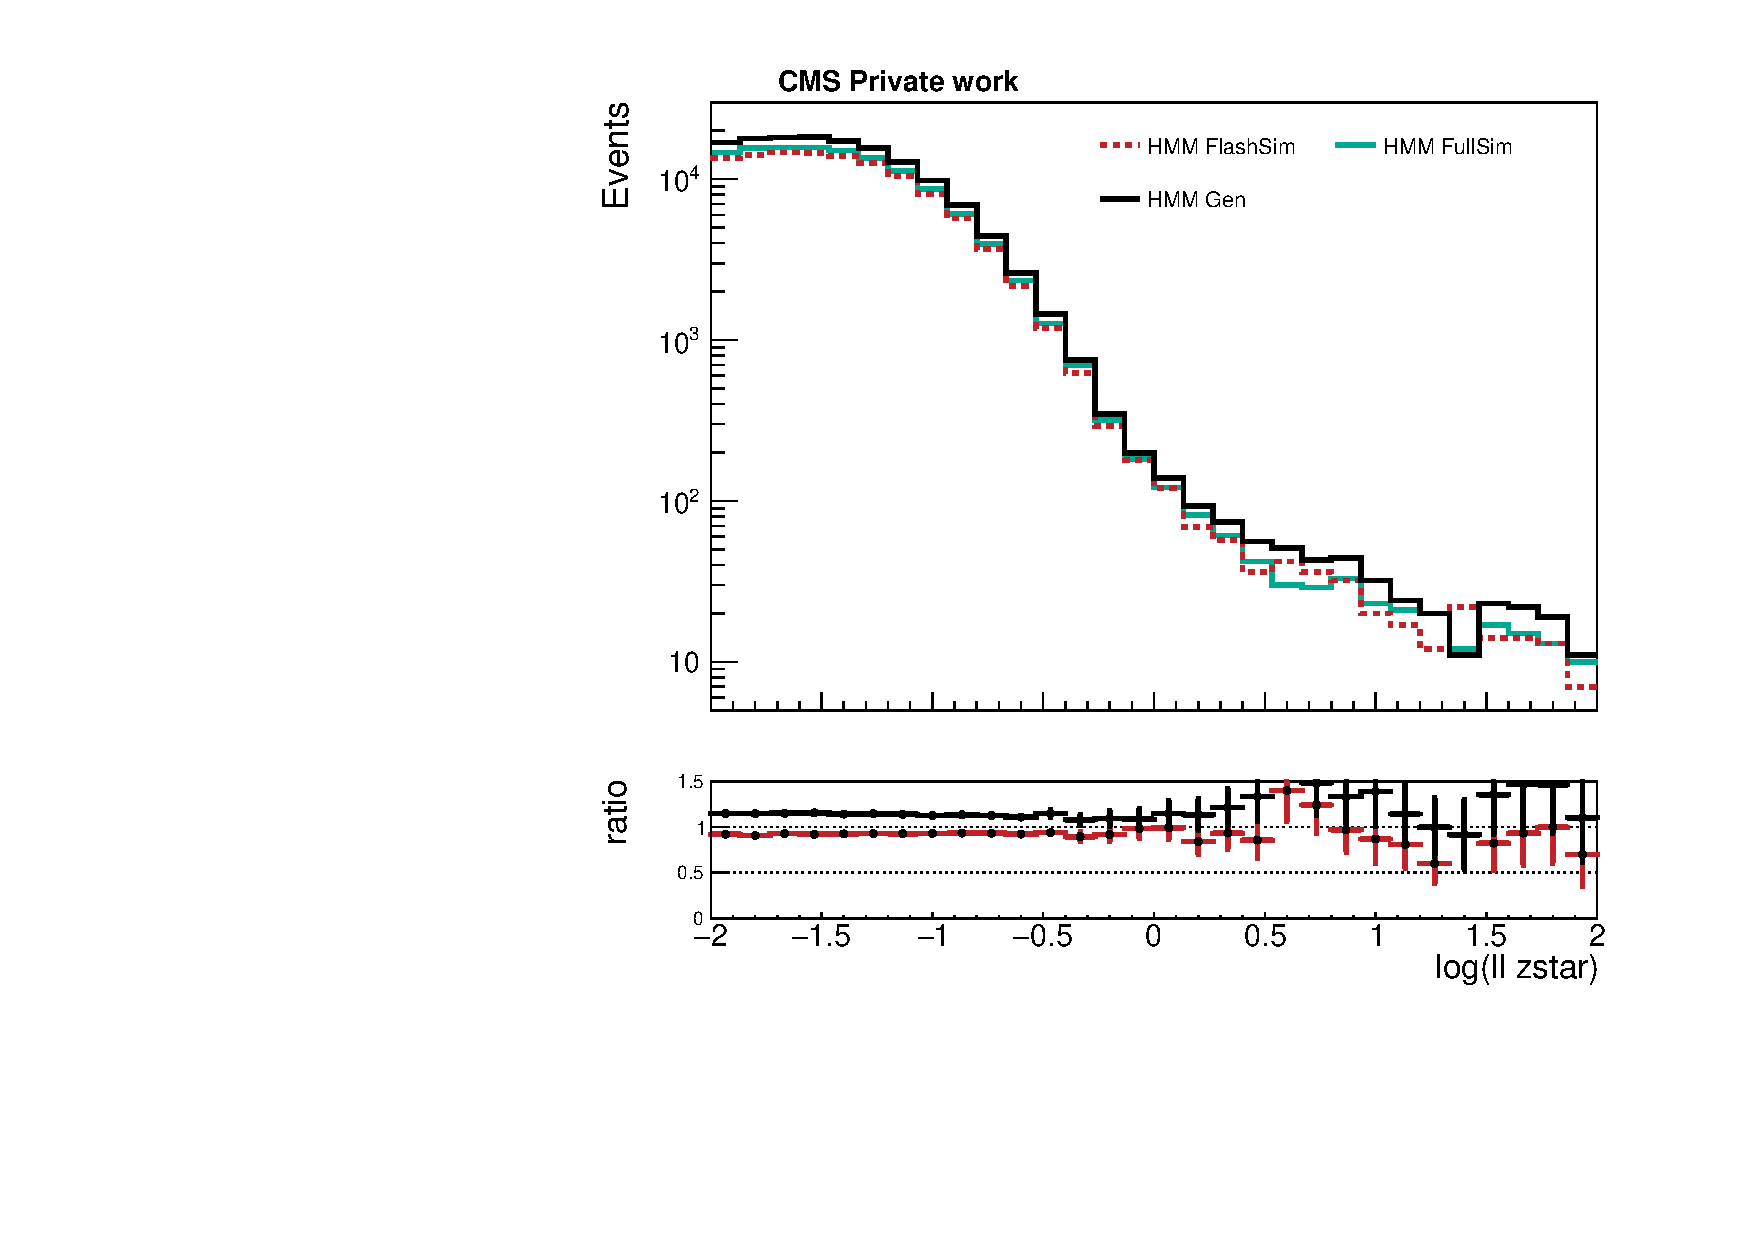
\includegraphics[width=\linewidth]{gfx/ch6/gen_vs_flash_ll_zstar_log___PreSel_log.pdf}
    \caption[Gen vs FlashSim for $z^*$]{Quantities depending on angular values, already very precise at Gen-level, show no significant deviation.}
    \label{fig:zstargen}
   \end{figure}
 
However, as we move to the $R(p_T)$, which depends on the hadronic activity, and thus on the effect of the interaction and reconstruction in the detector, we see the expected differences, as plot in Figure \ref{fig:rptgen}.

\begin{figure}
    \centering
    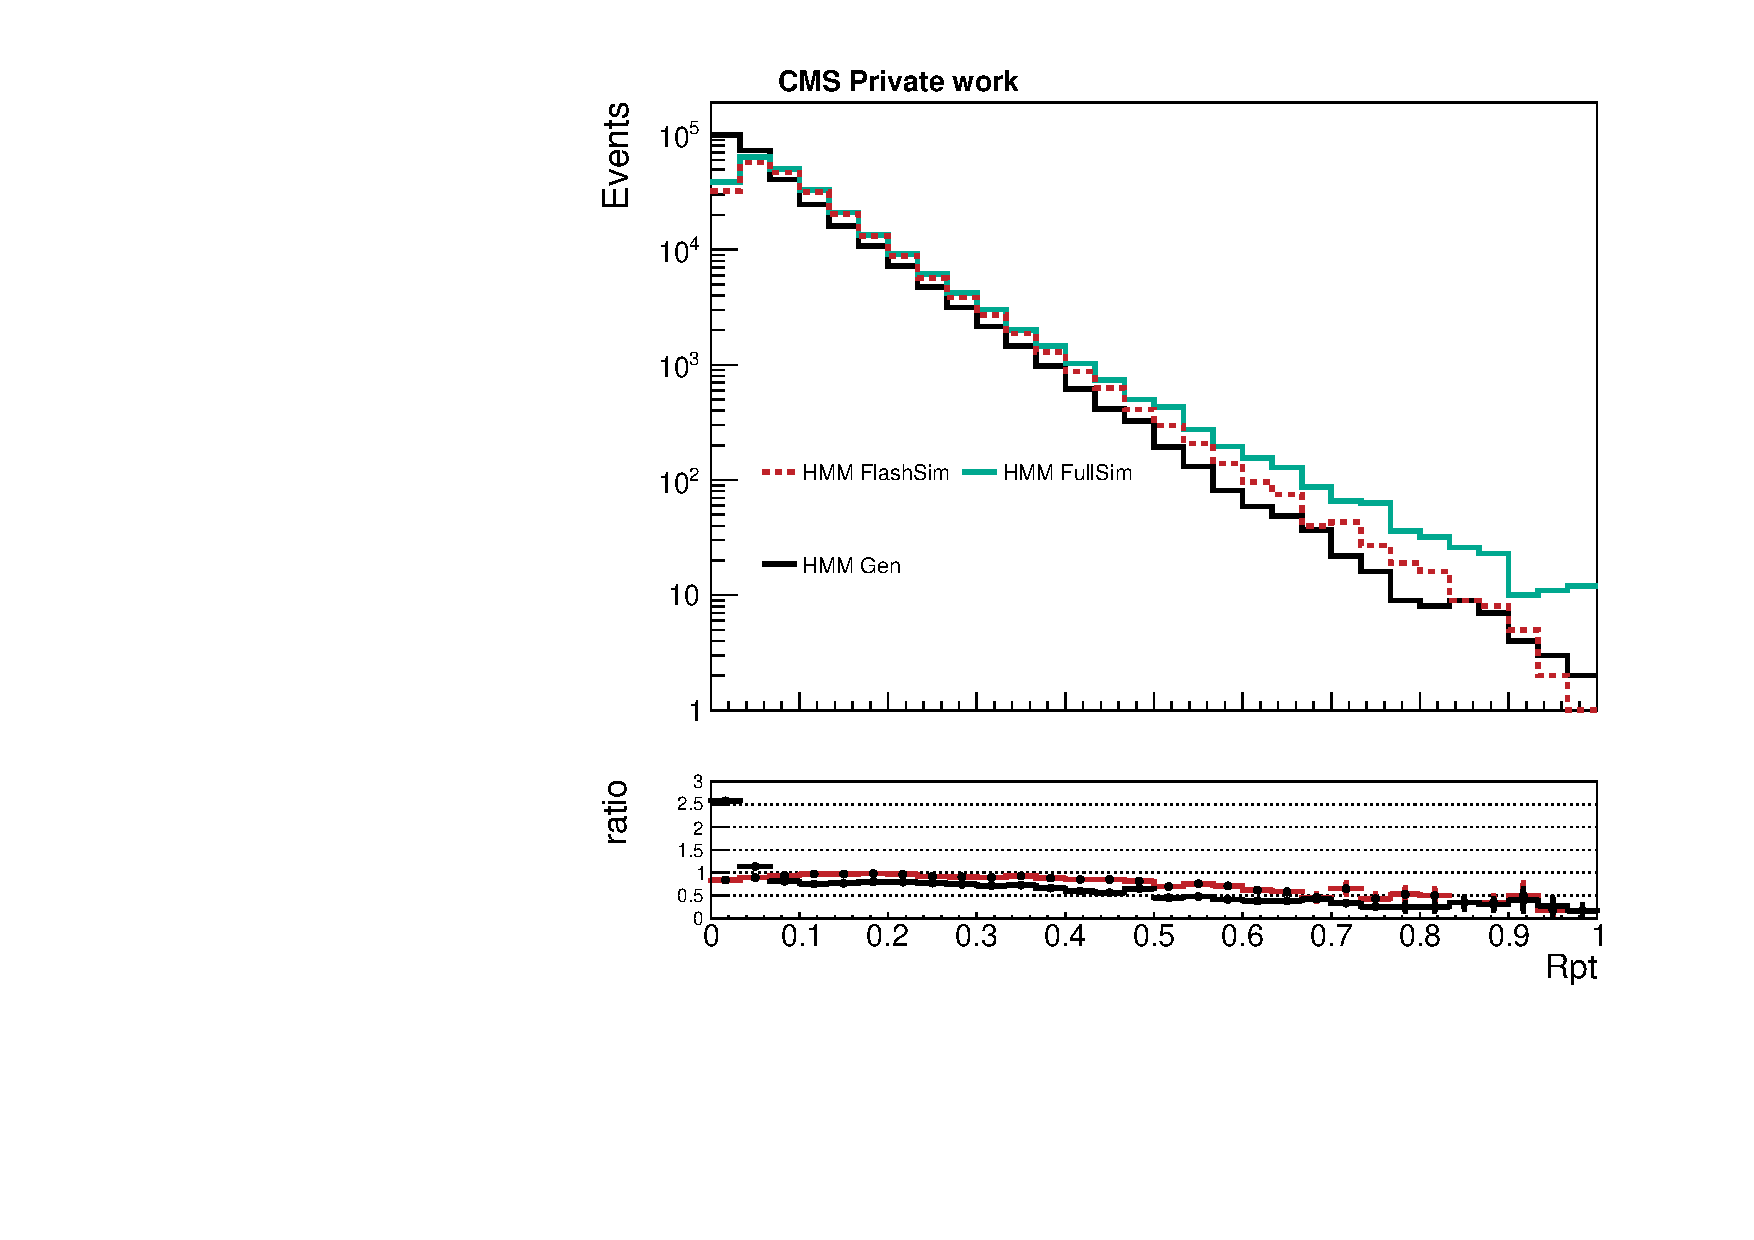
\includegraphics[width=\linewidth]{gfx/ch6/gen_vs_flash_Rpt___PreSel_log.pdf}
    \caption[Gen vs FlashSim for $R(p_T)$]{The dependence of $R(p_T)$ upon hadronic activity means that we start to see concrete differences between Gen and FlashSim.}
    \label{fig:rptgen}
   \end{figure}
   
The importance of the interaction with the detector and of the reconstruction, leading to \emph{smearing} in the distribution of the dimuon mass, is emphasized by Figure \ref{fig:higggen}, where we can see that the Gen has only a single, peaked value, while FlashSim has correctly learned the expected smearing.

\begin{figure}
    \centering
    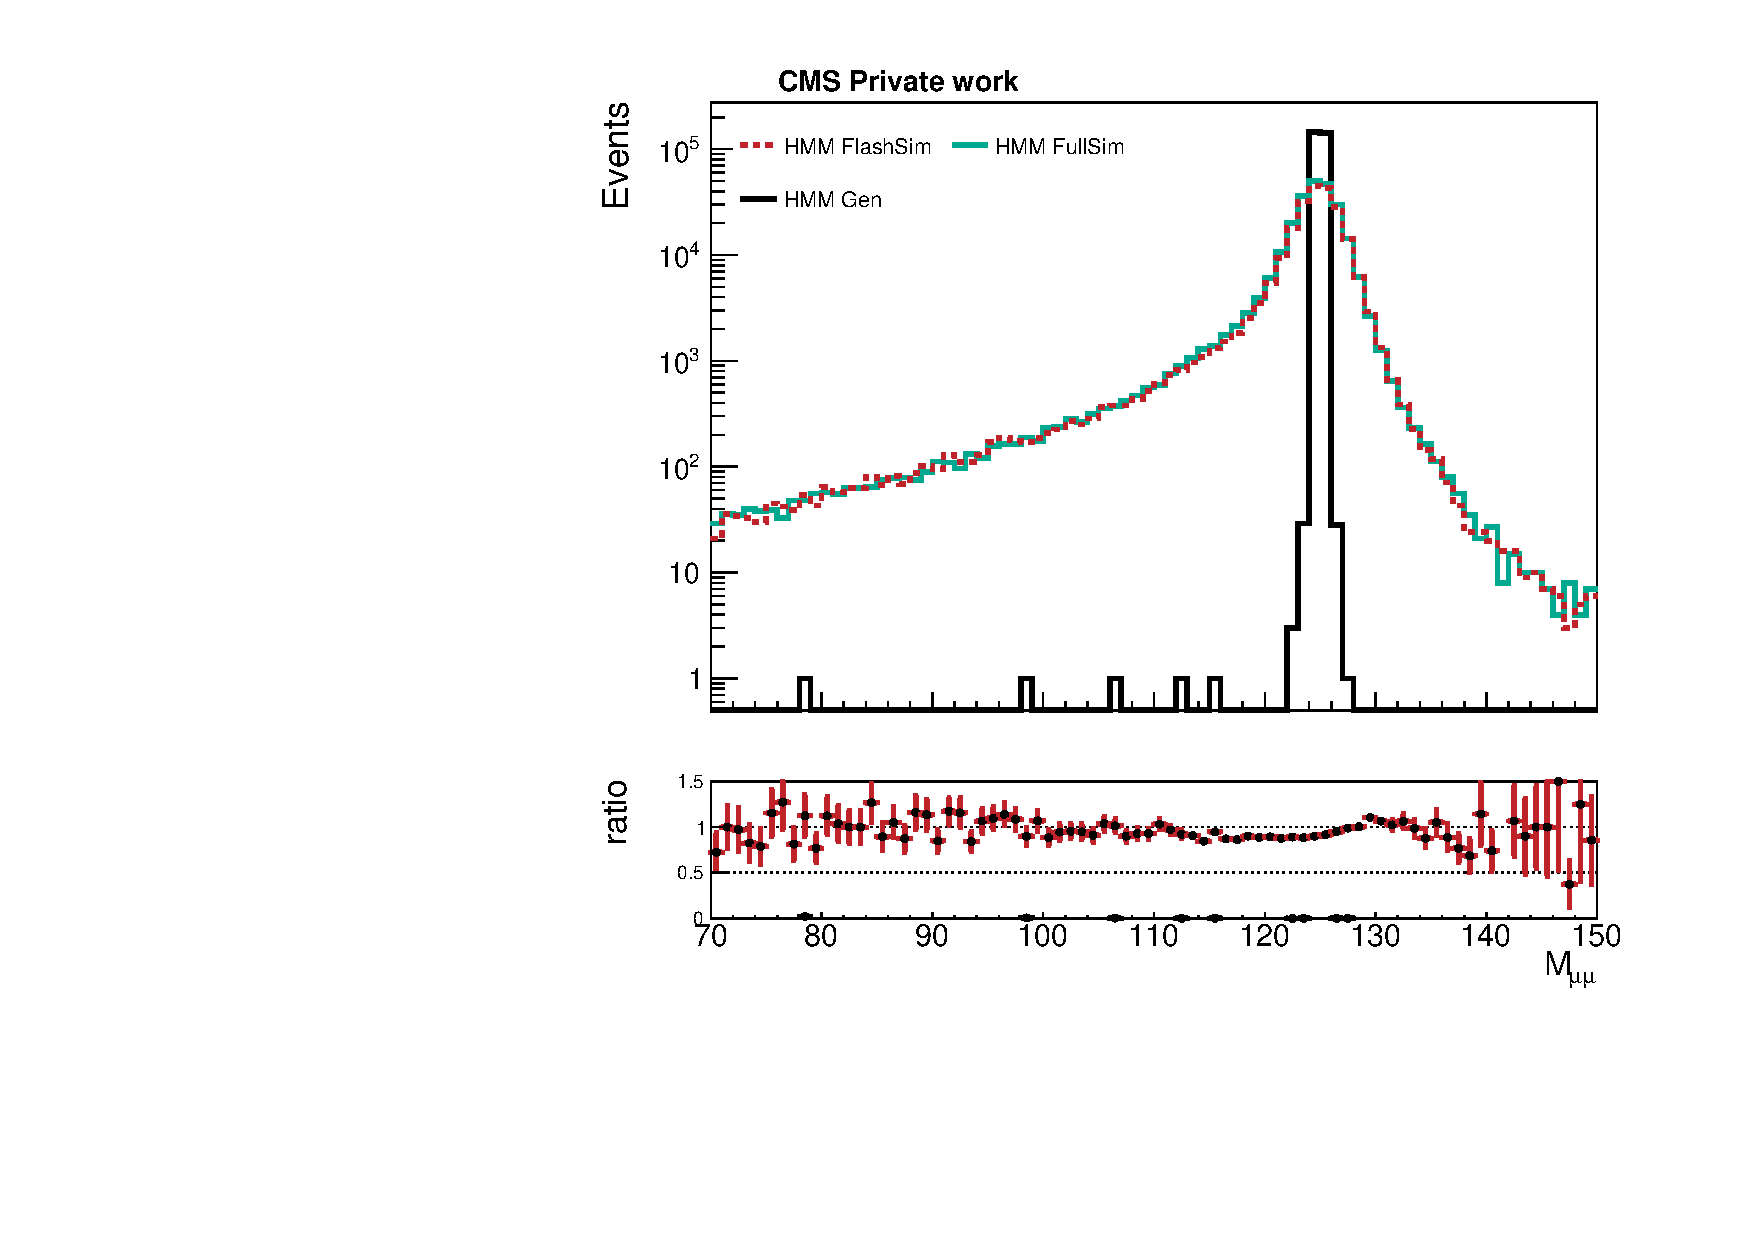
\includegraphics[width=\linewidth]{gfx/ch6/gen_vs_flash_Higgs_m___PreSel_log.pdf}
    \caption[Gen vs FlashSim for $M_{\mu\mu}$]{FlashSim has correctly learned the smearing due to the interaction with the detector and the reconstruction step.}
    \label{fig:higggen}
   \end{figure}
   
  Finally, this differences also translate to the crucial fit distribution of the VBF DNN Output, show in Figure \ref{fig:dnngen}.
  
  \begin{figure}
    \centering
    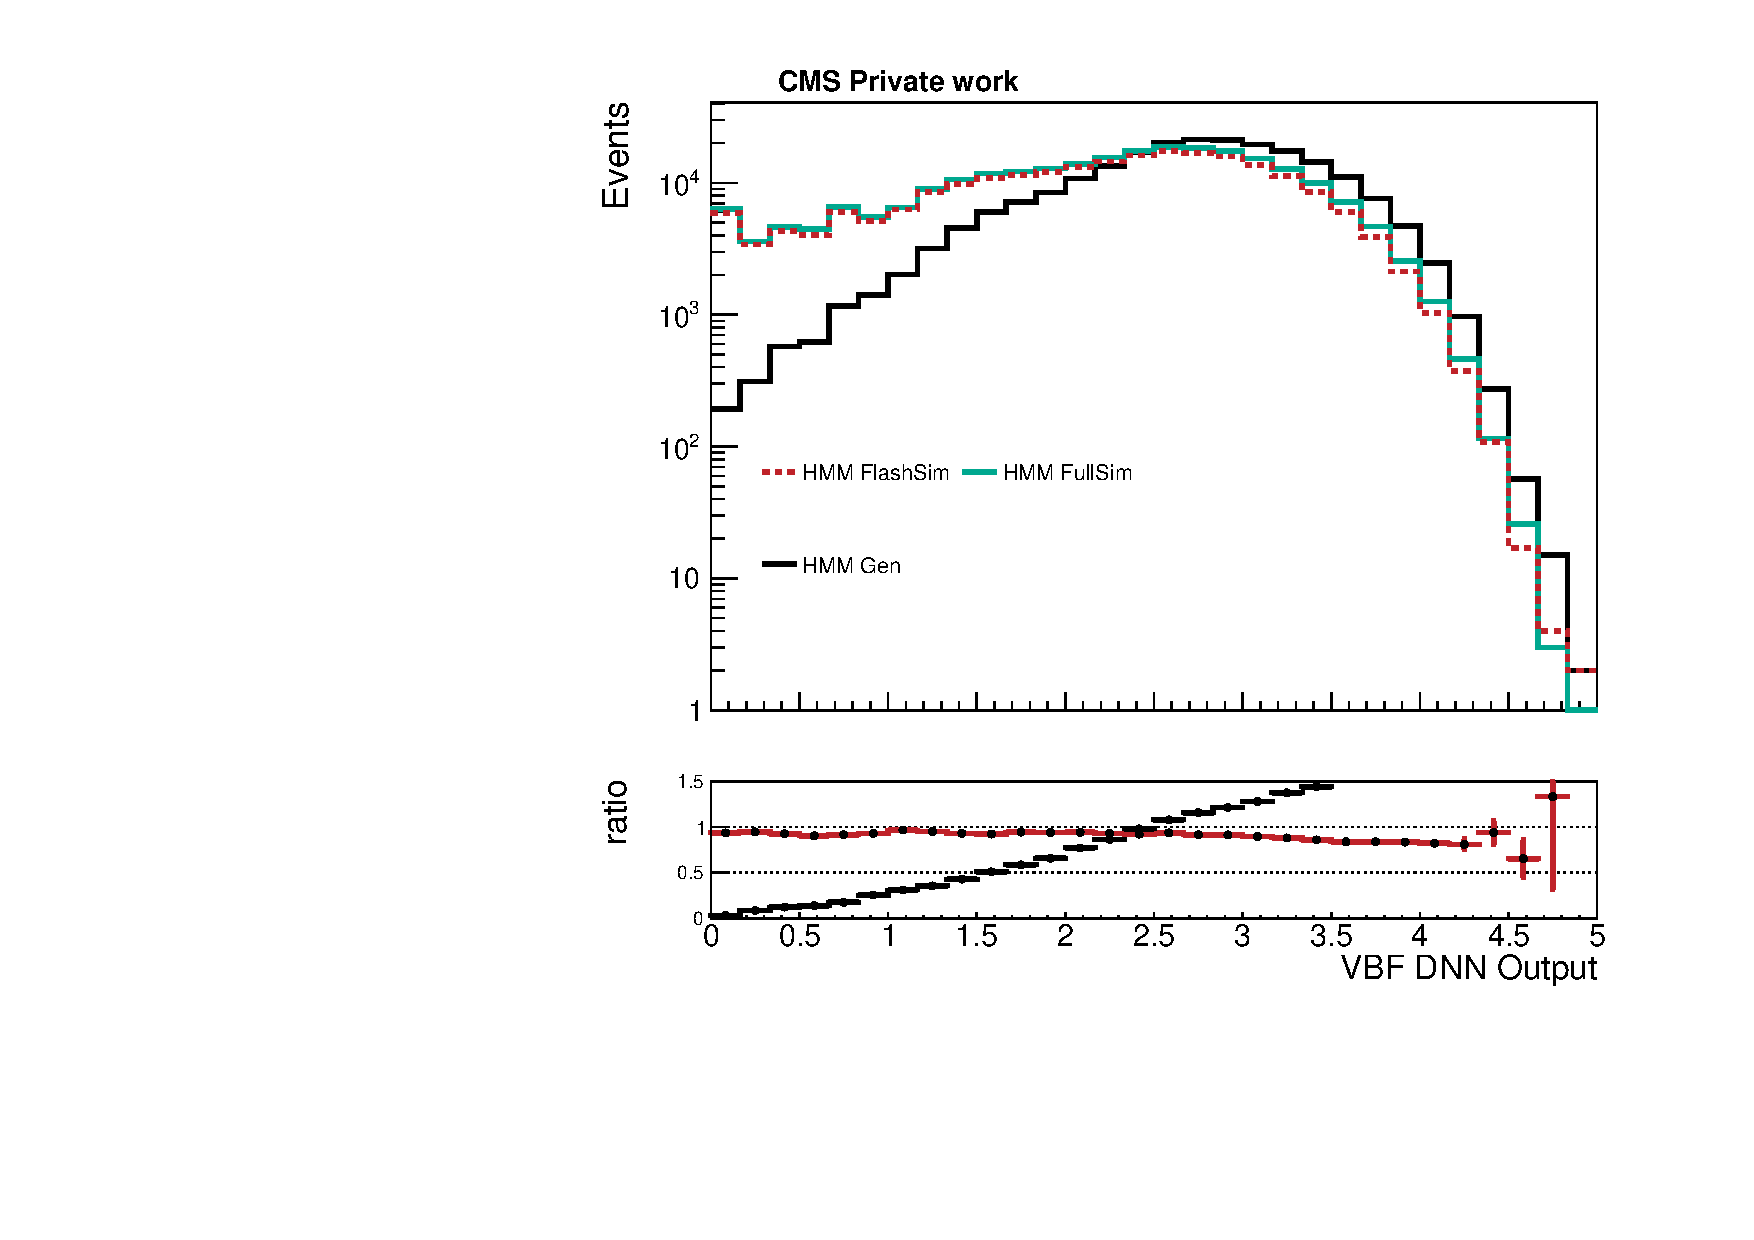
\includegraphics[width=\linewidth]{gfx/ch6/gen_vs_flash_DNN18Atan_noqgl___PreSel_log.pdf}
    \caption[Gen vs FlashSim for VBF DNN]{As expected, we observe a concrete difference between the Gen VBF DNN Output and those from FlashSim, which closely resemble the FullSim ones.}
    \label{fig:dnngen}
   \end{figure}
   
  These results of the present Chapter demonstrate that not only is FlashSim capable of producing different distributions from those of the bare Gen-level, but also that it can be used effectively in a real-world analysis scenario.